\chapter{Developed Peer-to-Peer Communication Prototype}
\label{chapter:work}

In this chapter the implementation of the developed peer-to-peer communication prototype will be analysed. This explanation will extend from the decisions of the technology and protocols to use to the architecture and workflow of the application.

It will begin with a brief summary of the steps taken to reach the developed application's features, functionalities and architecture. Which obstacles led to this solution and which were the fundamental drivers to decide upon this development and architecture to solve the problems previously stated. After the overall application's objectives and high-level architecture is described, a section on the lower-level architecture and components of the application will be presented, also containing flowcharts and diagrams on its normal functioning. A summary on the limitations and future work of this application will be given, as well as some possible solutions to its current limitations, outside the scope of this work. Finally, a conclusion on the difficulties and drawbacks of the development process and overall project appreciation will be given, along with some final thoughts on the work process and methods used.

\section{Peer-to-Peer Application Design Choices}

This section will provide the explanation and justification of the choices made for the application traffic type, ad hoc communication technology and ad hoc routing protocol.

In Section \ref{sec:wfd}, developed work on Android applications using Wi-Fi Direct has a mean of communication was introduced. Having the guidelines of these works in mind, the development of this application started. The main structure would always be: the application will have a routing algorithm that controls the destinations of the packets in each hop. A communication technology, \textit{e.g.} Bluetooth or Wi-Fi Direct, handler for both discovering nearby devices and establishing communication sockets with peers. A set of functions capable of analyzing incoming messages and deciding which is the next step to perform, in order to complete the requests/advertises. Finally, a user interface where the incoming messages can be seen and analysed (for debug purposes), also providing a text area for the user to enter the requested data.

\subsection{Application Type}

The choosing of what would be the transferred data between devices was one of the major steps of this work. Many ideas could be pursued and each one of them could be a great work to develop. The main contenders were text messages, beacon messages, geolocation messages and web pages. After some research was made, see Section \ref{sec:apps}, some of these contender could be eliminated, due to the existence of works already revolving around them. The main topic was text messages with many of the works developed focusing on recreating popular applications, such as Messenger and WhatsApp, using a peer-to-peer network to route the messages to their destinations. Beacon and geolocation messages were also not a completely innovative choice, since applications such as Uepaa!, see Subsection \ref{subsec:uepaa}, are already implementing systems similar to the one being proposed. Given this reasoning, the most innovative choice would be to transfer web pages between devices, creating a multi-hop hot spot in a peer-to-peer network.

\subsection{Ad Hoc Communication Technology}

After being established that web pages were the data to be requested, the next step was to choose the communication technology to be used, followed by the routing algorithm that would manage the next hops to take. The first and most obvious choice would be to use Wi-Fi Direct in both advertising and communication between devices, since this technology offers the best features to transfer files around 1Kbyte, in both range and data rate of transmission. However, during the development it proved to be impossible to continue with this approach, as Wi-Fi Direct's current Android implementation does not allow for devices to transfer files without user consent.

Given this drawback a shift to Bluetooth was made, and a hybrid version of the application was created, where the advertisement would be done via Wi-Fi Direct and the actual transfer of the web pages would be made via Bluetooth. This method also proved to be infeasible, due to security issues, since the the devices would have to display their Bluetooth MAC addresses in their Bluetooth name, making them much more vulnerable to possible attacks.

The advertisement was also a topic of debate. Two possibilities were presented: to use simple Bluetooth connections to advertise to each peer and to use \gls{BLE} beacons as an advertisement method. The first method is slower, since the advertising device needs to create a connection with each discovered peer, however it offers more security, since the receivers of the advertisement are targeted. Despite that, the second method would offer a better advertisement mechanism, since it is faster and consumes less resources than the traditional Bluetooth connections, see Subsection \ref{subsection:bt}, but it gives every device the ability of capturing the advertisement bringing some security issues.

The beacon advertisement is a tempting mechanism to implement, given all its advantages, it comprises two components: transmitting and ranging. Transmitting occurs when a device wants to issue an advertisement to a certain region\footnote{A beacon region is the physical space reached by the advertisement.}. Ranging is the act of listening to beacon transmissions in a certain region. During the implementation of this two components it was possible to verify that the current Android implementations - tested with Android versions 6.0 and 7.0 - are not able to reproduce \gls{BLE}'s transmitting mechanism, being only able to use the ranging.

Given these facts, the application was developed using Bluetooth for both advertisement of the devices and data transfer, although this is not the best technology for communication in a peer-to-peer network, it is the only one that, currently, meets all the requirements for this work. In the end of this chapter a brief discussion on the changes that need to be made to Wi-Fi Direct's implementation in Android will be presented, and why developers could benefit from these changes.

\subsection{Ad Hoc Routing Protocol}
\label{subsec:routprot}

The last step would be to create/modify a routing algorithm to control the destination of each incoming message. The requirements are simple, the algorithm simply needs to save the next hop of the shortest path leading to a device with Internet connection.

\gls{AODV} is a known routing scheme used in ad hoc mobile networks, precisely what this application will establish with the devices. However, it establishes dynamic paths, \textit{i.e.} only when a device wants to retrieve a web page does this protocol searches for a path in which to send the packet, see \cite{aodv} for the full specification of this scheme. This scheme is not the best for the applications reliability, since the requesting device should know before hand if it is capable of reaching the Internet, otherwise users will experience long periods of path requesting and advertising every time they request a web page.

\gls{DSDV} is also known for its use in ad hoc mobile networks. This protocol uses a routing table where it stores in each entry: the destination, next hop, number of hops to reach the destination and a sequence number - avoiding routing loops. The devices exchange full routing tables, creating a network where every device has total knowledge of the topology, being a powerful advantage. However, \gls{DSDV} requires the exchange of routing tables and their regular updates, using unnecessary bandwidth, see \cite{dsdv} for more information on \gls{DSDV}.

Since the routing of this work does not have a specific destination as a goal, in other words, device A does not want to transmit to B, it only wants to reach a node with network access with the minimum amount of hops, so A does not have knowledge on where its message will be sent after the immediate next hop. Thus, in order to accommodate such requirements some modifications were made to \gls{DSDV}. Firstly, to reduce the bandwidth used by \gls{DSDV}, this adaptation will simply exchange the best estimate of the current device, only including the number of hops and the device's \gls{MAC} address. Secondly, instead of a periodic exchange of tables, devices will update their tables every time a new advertise message is received and they only exchange routing information when a new best path is received, with the contents described above.

\section{Architecture}
\label{sec:architecture}

In this section the architectures of both framework and application are presented. It will consist of: a description of the Bluetooth connections between devices, an explanation on the discovery and advertising mechanism and a analysis of the web page exchange process.

\begin{figure}[ht]
	\noindent\makebox[\textwidth]
	{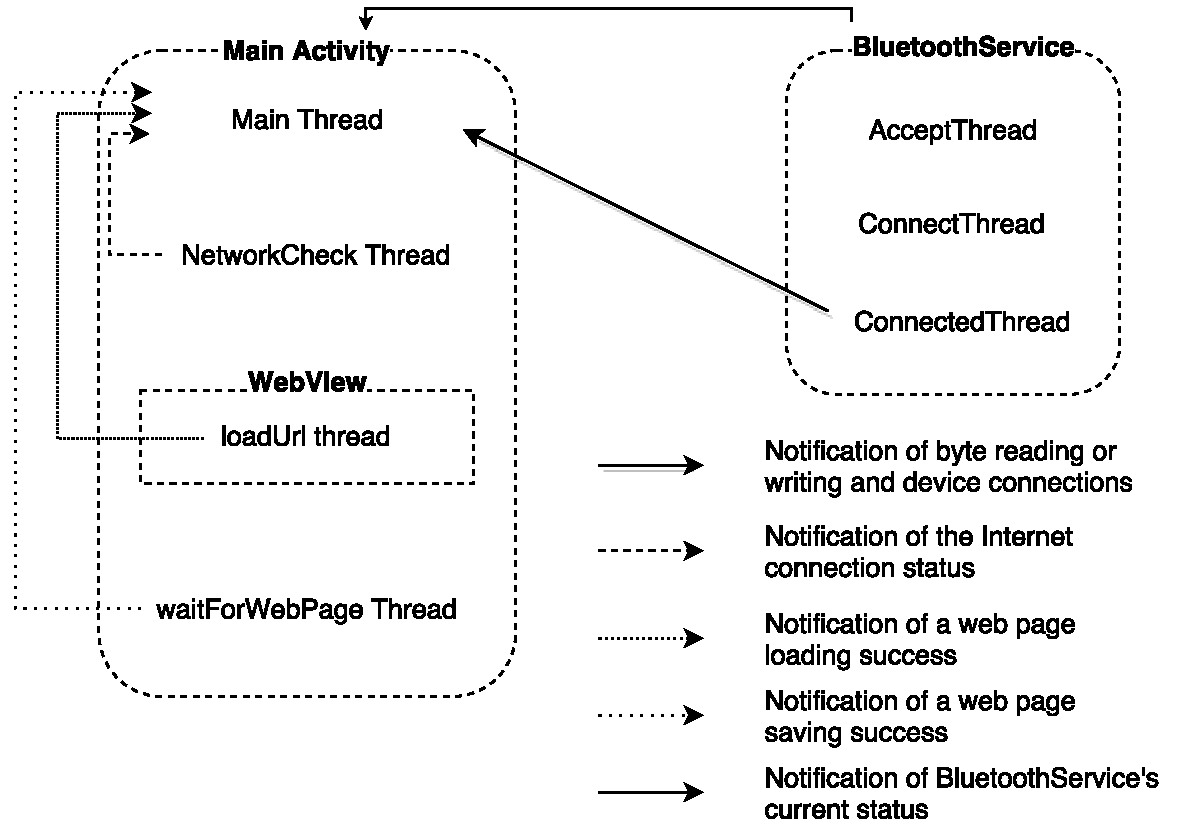
\includegraphics[width=1\textwidth]{images/app_sandbox.pdf}}
	\caption{\label{fig:appsandbox} Overview of the different parts of the application and the communication between the threads running in each part}
\end{figure}

In Figure \ref{fig:appsandbox} an overview of the application is shown. It can be seen that there are two main parts of the application, the main activity and the \textit{BluetoothService}.
\begin{itemize}

\item The main activity is where most of the processing logic is executed, from the analysis of the received data to the management of the routing tables, it comprises of four threads: the main thread seen by the user, also known as the user interface thread. The \textit{NetworkCheck} thread used to perform the query regarding the Internet connection status of the device. The \textit{loadUrl} thread, created when a \textit{WebView} object is used to show or download a web page. Finally, the \textit{waitForWebPage} Thread used to ensure the requested web page is successfully saved in the device.

\item The \textit{BluetoothService} is used to manage the Bluetooth connections between devices, it is composed by three threads: the \textit{AcceptThread}, the \textit{ConnectThread} and the \textit{ConnectedThread}. Each of these threads will be explained in detail in the next subsection.

\end{itemize}

Inside the main activity the different threads communication with each other, mainly to notify the main thread of a certain occurrence that may lead to a new set of actions. However, communication is also done between the main activity and the service , usually when the first needs to access the \textit{BluetoothService}'s current status.

Having a better understanding on how the application is divided and the communication between the different parts the next subsections should be more easily comprehended.

\subsection{Bluetooth Connections}
\label{subsec:btconn}

In this subsection the Bluetooth connections between devices and their possible stages will be described and analysed.

Since the communication technology is Bluetooth, the application must have a thread\footnote{Thread is a sequence of instructions managed independently, usually by a scheduler from the operating system, see \cite{threads} for more documentation on threads.} that handles the listening and acceptance of connections and the data transfer between devices. This corresponds to the \textit{BluetoothService.java} class, from the application. It creates and listens to insecure communication sockets allowing devices to exchange data without user approval.

The service has three different threads within it: a thread for the acceptance of incoming communications - \textit{AcceptThread}, a thread for the initial exchange of vital information before the connection - \textit{ConnectThread} - and a thread for the actual exchange of data between devices - \textit{ConnectedThread}. The connection of devices goes through each of these stages, allowing the main thread to get information on what is the connection status of the device at a given time.

There were two different approaches to the connections of devices: either the devices stayed connected as long as possible until a new connection was requested or the devices stayed connected for the minimal amount of time for data to be transferred. The second approach was used, since it is the one that is more energy efficient, draining a lower amount of battery from the devices.

Bluetooth communication between devices is only allowed if both devices have matching "credentials", providing a minimum amount of security to prevent against possible attacks. An application specific name and \gls{UUID} represent the application, making it distinguishable from any other, since the \gls{UUID} of an application should not be repeated in any other.

To notify the main thread of what is being done by the \textit{BluetoothService} a handler is created, acting as bridge between the two parts. It can be used for various actions, such as: retrieving the status of a connection, assessing if a device is ready to receive a file, \textit{etc.}

To substantiate the possible Bluetooth connections stages four different textual representations are defined, one for each stage: listening, connecting, connected and not enabled. Each type of thread mentioned earlier is associated with one stage, being the non-existence of a thread the not enabled stage. The different threads can be seen as the implementation of a stage. They are the ones that dictate how is the application going to act during the stage. 

In the next subsections each stage will be explained in detail, providing a better understanding on how the connections are performed.

\subsubsection{Listening}
\label{subsubsec:listening}

A device is said to be in the listening stage when it has no ongoing connection but it is waiting for a new one initiated by another device. It is the "first" stage of the \textit{BluetoothService}, since every time the service is initiated the device is moved to this stage.

As was said previously, each connection stage is associated with a thread class. The listening stage is associated with the \textit{AcceptThread}, which is instantiated every time the device enters this stage. The framework's connections have short durations and each time a new connection is performed the service is restarted, entering the listening stage. Hence, it is imperative to assure there are no memory leaks or communication sockets left open. Thus, before the listening thread is instantiated it is verified if any other Bluetooth connection threads are running and, if so, they are shut down.

Once all the requirements for the instantiation of a new thread are met, a communication socket is created with which the device listens to incoming communications. To implement the listening mechanism a loop is created whose purpose is to block the thread until a new connection is received, an error occurs or the user shuts down the application.

Whenever the device receives a new connection, it verifies the "credentials" sent in that request and compares them with the ones defined in its \textit{BluetoothService}. If they match the connection is accepted.

Upon successfully accepting a connection, the method assesses the status of the newly formed connection and decides upon it. If everything goes as planned, the connection should now be in the connected stage. Once this migration between stages is concluded the instance of the listening thread is destroyed, for reasons above stated and the 

\begin{figure}[ht]
	\noindent\makebox[\textwidth]
	{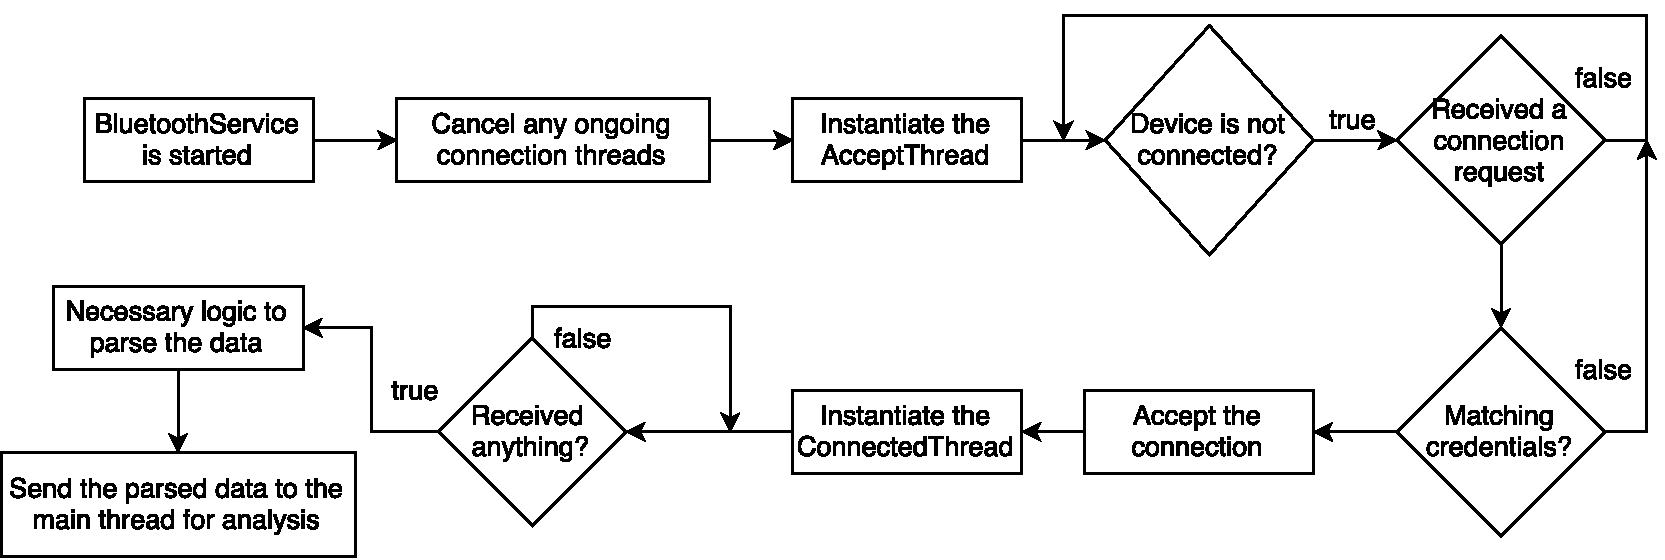
\includegraphics[width=1\textwidth]{images/btreceiver.pdf}}
	\caption{\label{fig:btreceiver} Fluxogram of a Bluetooth connection receiver's performed actions}
\end{figure}

In Figure \ref{fig:btreceiver} it is possible to see the performed actions from the point of view of a device that is waiting for incoming connections. It starts when the \textit{BluetoothService} is initiated and finishes when the received bytes are sent to the main thread for analysis, described in \ref{subsubsec:connected}.

\subsubsection{Connecting}
\label{subsubsec:connecting}

Concluded the listening and accepting of connections it is necessary to understand how they are requested. For a Bluetooth connection to be performed at least two devices must exist, one of them acting as the connection requester.

Similar to the listening thread initiation, the \textit{ConnectThread} is only instantiated after all the previous Bluetooth connection threads running in the device are shut down. Also, to avoid delays during the connection process, the Bluetooth discovery process is shut down. Only then can the requester attempt to establish a connection with the desired device.

To identify the receiver of the connection request, the device needs to retrieve the \gls{MAC} address of its counterpart, this will be explained in Subsection \ref{subsec:disandadv}. Once this is attained the requester can attempt to create a communication socket between both devices, using the previously defined Bluetooth "credentials" and the receiver's \gls{MAC} address. If the \gls{MAC} address is valid and corresponds to a device within reach the connection is request successfully.

In case of failure due to the rejection of the connection from the receiver, a notification is sent to the main thread, notifying the connection was not successful and the service is restarted.

However, if the sent request is accepted by the receiver, the connection state is assessed and, if no interruptions or errors occur, the connection stage is moved to the connected stage, indicating both devices are able to send and receive bytes from their counterpart, by writing and reading from the established communication socket, respectively.

\begin{figure}[ht]
	\noindent\makebox[\textwidth]
	{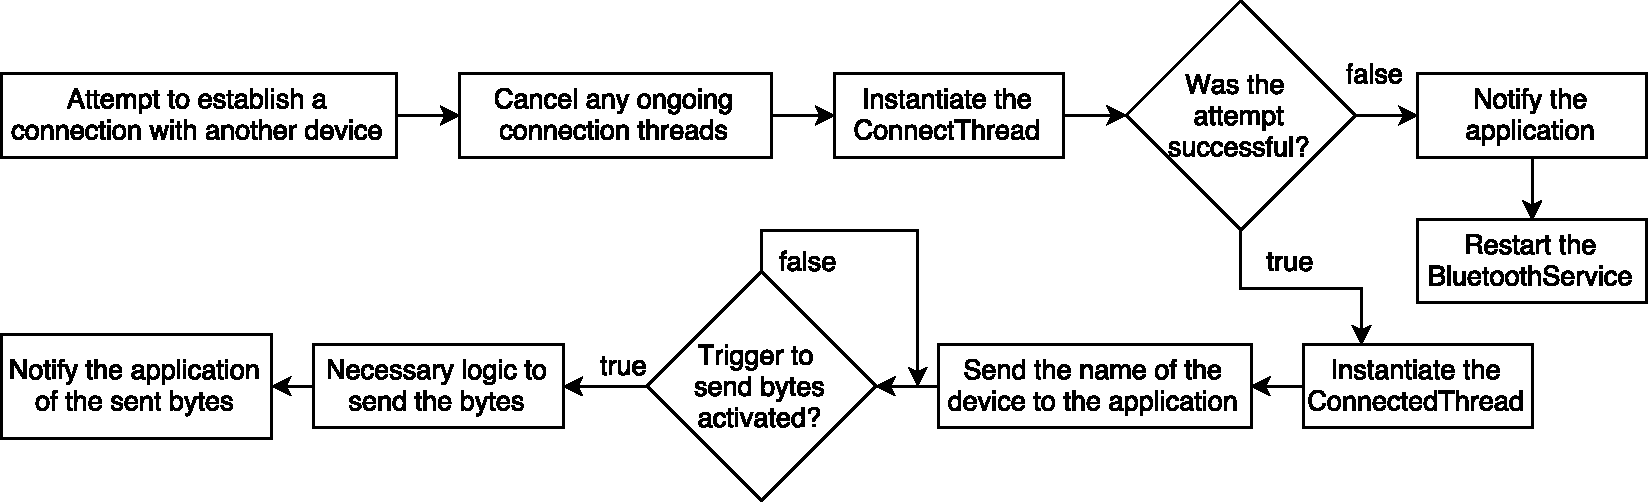
\includegraphics[width=1\textwidth]{images/btrequester.pdf}}
	\caption{\label{fig:btrequester} Fluxogram of a Bluetooth connection requester's performed actions}
\end{figure}

In Figure \ref{fig:btrequester} the actions performed by a Bluetooth connection requester can be seen. Beginning by the attempt to establish a connection to the notification of the successfully sent bytes, described in the next subsection.

\subsubsection{Connected}
\label{subsubsec:connected}

When the connection reaches the connected state both requester and receiver devices are linked through a Bluetooth communication socket. To start the receiving and transmitting mechanisms a \textit{ConnectedThread} is created, after all ongoing threads are cancelled to avoid conflicts between communications or memory leaks. To notify the main thread of the connection success the service sends the counterpart's Bluetooth identifier, \textit{i.e.} its Bluetooth name, to the main thread.

To understand how data is transferred between the two connected devices it is necessary to explain two different mechanisms: the writing of data and the reading of data. By creating a socket linking both devices two data streams are also created, implicitly, where one provides a stream to write data into the socket and the other provides a stream to read data from the socket, see Figure \ref{fig:inoutstreams}. Both writing and reading data is in the form of byte arrays that can be posteriorly manipulated into the desired format.

\begin{figure}[ht]
	\noindent\makebox[\textwidth]
	{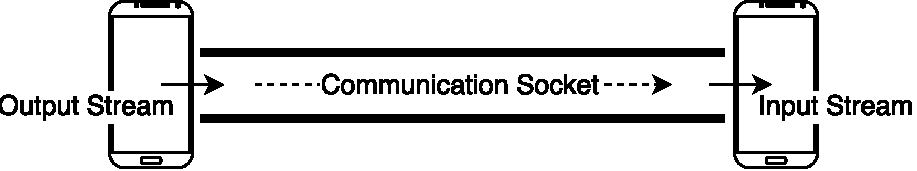
\includegraphics[width=0.8\textwidth]{images/inoutstreams.pdf}}
	\caption{\label{fig:inoutstreams} Communication channel with input and output streams}
\end{figure}

The writing of bytes into the socket is done through an output stream, name given to the part of the stream that handles the writing. For any data format the principle is the same, to convert the data into a byte array that will be sent through the stream. It is important to note that the channel has a limited size buffer shrinking the arrays' size, thus if the data to be exchanged has a large amount of bytes, it is wise to create a cycle that sends parts of that data, instead of the whole. The writing process is asynchronous, since it is only executed at a certain time following a certain trigger, \textit{e.g.} user input. It is possible to notify the main thread of the sent bytes if they are relevant to other processes, \textit{e.g.} notifying that a text message was sent and prepare to receive/send an image.

The reading of data from the socket is done through an input stream. Since the output stream only writes byte arrays into the socket the input stream will only read byte arrays. This property burdens the developer with the task of treating the received bytes, \textit{i.e.} converting them to their original data type. Also, as mentioned before, the communication socket has a limited size buffer, thus it is also the developer's responsibility to create the reception cycle, following the premises used to create the sending cycle, \textit{e.g.} read the same amount of bytes sent. This mechanism may need to comprise the necessary logic to aggregate the multiple byte arrays received, if the original data was divided and sent in several parts. The reception loop is running while the connection remains active and whenever bytes are read from the socket, these are sent to the main thread to be analysed and converted back to their original format.

To send and receive different data formats within the same application it is needed to develop a protocol to handle the different conversions of the sent and received byte arrays. Further along this chapter it will be explained how this was done in the developed application to exchange both text messages and web pages.

\subsection{Discovery and Advertising}
\label{subsec:disandadv}

Now that the basic concepts on how the communication between devices are implemented are explained, it is possible to dig deeper into the intrinsics of the application itself, and what is the logic behind the routing of web pages.

The first thing in order for each device to know what is the next hop of a certain request will be to fill the routing tables. This process is done by a series of discoveries\footnote{Discovery is the act of finding nearby devices with Bluetooth on.} and advertisements\footnote{Advertise is the act of notifying peer devices of the cost of relaying a request to the device issuing the advertisement.}. Upon starting the main activity, each device will advertise its best estimate to reach the Internet. This advertisement will be received by peers and analysed. In case the estimate of relaying the requests through that node improves the current estimate, the receiving peer will begin another discovery and advertising process with the newly discovered path. Otherwise, the peer will add or update an entry in the routing table, regarding the advertiser.

\begin{figure}[ht]
   \noindent\makebox[\textwidth]
    {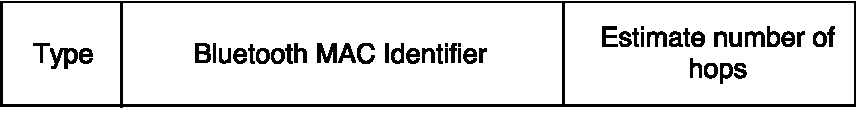
\includegraphics[width=0.7\textwidth]{images/adv_message.pdf}}
	\caption{\label{fig:advmsg} Advertising message format}
\end{figure}

In Figure \ref{fig:advmsg} the format of an advertise message is shown. The type is a feature common to all messages exchanged in this application. It servers the purpose of identifying which type of message is being received. It can take four different values: \textit{ADV}, \textit{RQT}, \textit{RSP} and \textit{FAIL} for an advertisement, request, response and fail message, respectively. In this case it will take the value \textit{ADV}. The delimiters of the different message parts - vertical lines in Figure \ref{fig:advmsg} - are represented by the dot comma character (;), in order to be able to separate the different parts of the message. The Bluetooth \gls{MAC} identifier is always the \gls{MAC} address of the Bluetooth adapter of the sender, it is then used by the receiver to populate its routing table. Finally, the estimate number of hops is the smallest number of hops the sender needs to be able to reach the Internet plus one, corresponding to the hop from the receiver to the sender.

Each device has two different routing tables: one that is used to store the information retrieved from the advertisement process, providing the best path for routing the requests to the final device. Other that is used to route the responses back to the original sender, as explained in the next subsection. For simplicity the first routing table will be referred by the same name, while the second will be referred to as response table, as it handles the routing of responses. 

Both routing and response tables along with some other variables, such as the one keeping the Internet access state must be made accessible and synchronized throughout the application. Hence, contrasting to other variables they can be referred to as application specific.

\begin{table}[ht]
\centering
\bgroup
\def\arraystretch{2.5}
\begin{tabular}{|c|c|}
\hline
\textbf{Next hop's MAC} & \textbf{Number of hops} \\ \hline
Own MAC & 0 or 16 \\ \hline
Device A's MAC & Estimate through A \\ \hline
Device B's MAC & Estimate through B \\ \hline
... & ... \\ \hline
Device Z's MAC & Estimate through Z \\ \hline
\end{tabular}
\egroup
\caption{Routing table example and format}
\label{tab:routTables}
\end{table}

In Table \ref{tab:routTables}, an example of a routing table is presented, where the first entry is always populated with the device's own \gls{MAC} address and its estimate, which is either 0 or 16\footnote{16 was chosen to be the representation of infinity or inability to reach a destination, since it has been represented by this number in various protocols, for instance in \gls{RIP}, see \cite{ripprotocol}}, meaning the device has an Internet connection or not, respectively. Every time a device receives an advertisement message, it populates this table, either by adding a new row or updating an existing one, with the information contained in the message - see Figure \ref{fig:advmsg}. When the routing table is done being populated, each node knows its immediate peers and the best estimate through each one of those peers, giving it a full knowledge of its vicinity, \textit{i.e.}, the sub-network created by the peers that are reached by the device using a single hop.

It is important to start by understanding how the routing tables are created and, posteriorly, how and when they are populated. Both tables follow the same principle, they are objects that relate keys to values. To a single key corresponds a single value, thus not creating duplicate entries.

In the scope of this subsection only the routing table will be explained, see Subsection \ref{subsec:exch} for the description of the response table. The keys of this table correspond to the \gls{MAC} address of the next hop while the values correspond to the respective estimated number of hops. So when querying the table for a specific \gls{MAC} address it should return one and only one estimated number of hops.

There are three important features that the application needs from this table: to get the absolute minimum value, meaning retrieving the lowest possible value for any given key, in order to retrieve the device's best path. To get the corresponding key to the minimum value, in order to retrieve the receiver to whom this device should send the message. Finally, to update or add a row with a new key-value pair, in order to add newly received advertisement information.

To be able to get the absolute minimum of the estimated number of hops, it is necessary to compare all the existing values of the table. Since it only contains the information of its immediate peers this process is fast and does not interfere with the rest of the application. However, if the routing table keeps the information from all the devices in the network, as suggested in \textit{DSDV}, see Subsection \ref{subsec:routprot}, this could be a heavy resource consumption process and could impact the well functioning of the application. If the routing table comprises a minimum estimated number of hops that value will be returned. However, if the table is not populated, 16 will be returned, for reasons explained above.

Having the minimum value from the routing table, it is now necessary to retrieve the \gls{MAC} address corresponding to the device providing this estimate. This is done by iterating through every key and, in every iteration, comparing the value of the current key to the minimum value, previously defined. If, in a given iteration, it finds a key mapping the desired value, this key will be returned, corresponding to \gls{MAC} address of a device that gives the minimum estimated number of hops, otherwise the main thread must be notified that there is no best estimate. It is important to note that several devices may provide the shortest path, but the application will only choose the one that was found first, since they all provide the same estimate.

\begin{figure}[ht]
	\noindent\makebox[\textwidth]
	{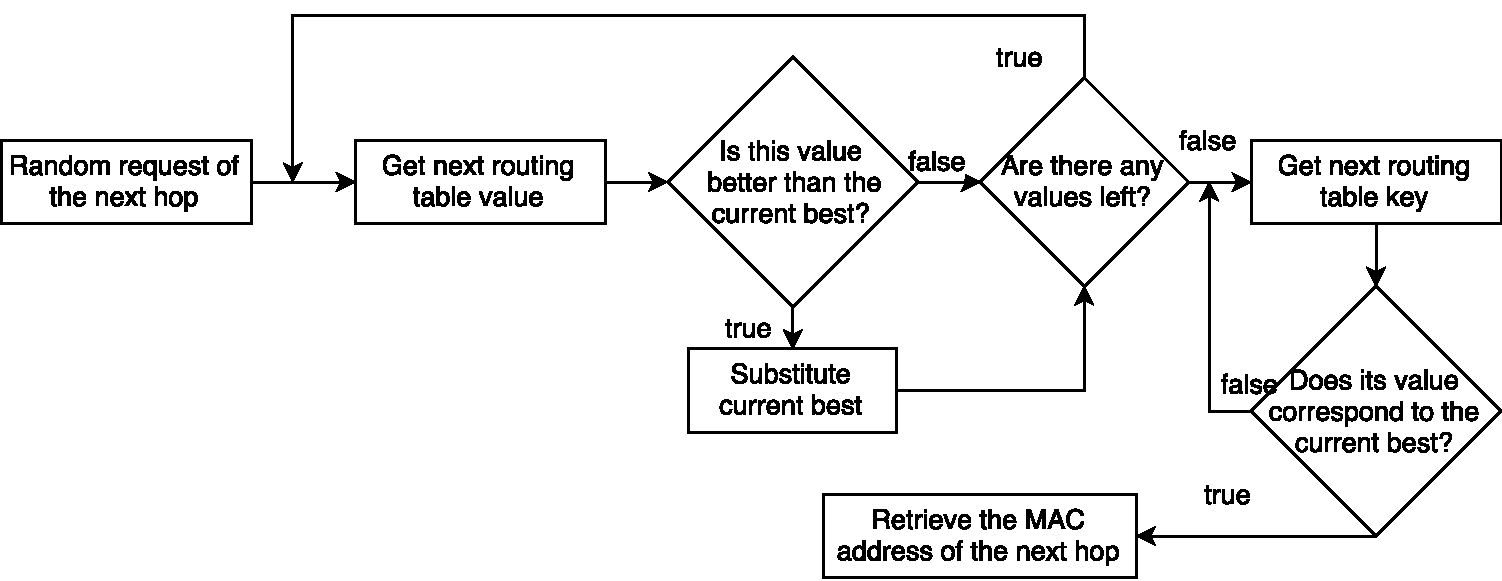
\includegraphics[width=1\textwidth]{images/nexthoprqt.pdf}}
	\caption{\label{fig:nexthoprqt} Process of retrieving the next hop from the routing table}
\end{figure}

In Figure \ref{fig:nexthoprqt} it is shown how the application proceeds to retrieve the \gls{MAC} address of the next hop where a new request will be sent. It contains two main loops, one iterating through all the values in search of the lowest and one iterating through all the keys to find one that maps to that value.

Finally, the addition and update of routing table rows is done whenever an advertisement message is received. By separating the message in its parts, according to Figure \ref{fig:advmsg}, it is possible to retrieve both the \gls{MAC} address and estimated number of hops through that peer. Having this information it is possible to insert the retrieved key-value pair into the existing table. As mentioned before one key maps to a single value, thus in case this key already maps to a value, the latter will be overwritten with the new one. In case the key does not exist a new row is created mapping the key to its specific estimate. Note that, in case of a table update, the application does not compare values, \textit{i.e.}, it does not check if the new estimate is better than the old one, since the sender device could have lost the communication with the best route and thus it needs to advertise a worse path. If this check was made, the receiver could be mislead into sending requests through this device, thinking it would provide the better path.

\subsubsection{Discovering Peers}
\label{subsubsec:disc}

Now that it is clear how the mechanism of modifying the routing tables works, it is possible to discuss where and when these methods are being called. However, before that there are still some indispensable features that need mentioning:

\begin{itemize}
	\item During the peer discovery process several peers may be found, making it necessary to create a place to store them, for further examination. To achieve this a list of Bluetooth devices is created, where each device corresponds to a found peer in the discovery process. This list is then used to retrieve information from these devices, in order to successfully establish communication sockets with them.
	
	\item To prevent the discovery process of dragging for longer than expected, using processing resources and damaging the performance of the rest of the application, it is necessary to identify if this process is finished and notify the main thread.
\end{itemize}

Before beginning the discovery process the application needs to ensure all the conditions are met. The Bluetooth status is the first to be checked, the device should have Bluetooth enabled and it should be discoverable for an unlimited amount of time. If the Bluetooth is not enabled the device cannot begin the discovery process and if the device is not discoverable its peers are not able to make their advertisement reach it.

Once the Bluetooth is set up, the initial update of the routing table is performed, a quick network check indicates if the device has an active Internet connection. Should the check return positive, it will add a new row to the routing with its own \gls{MAC} address and 0 hops, since its estimate to reach the Internet is immediate. In case the check returns negative, meaning the device is currently unable to establish an Internet connection, the same process is performed, however instead of 0 hops, the estimate will be of 16 hops, for reasons already explained.

The device is now finished with the first step of advertisement, filling the routing table with its own \gls{MAC} address and estimate. It is now possible to start the discovery process to advertise this same estimate to the discovered peers.

Figure \ref{fig:adveg1} demonstrates how two devices, one without an Internet connection (left) and one with an active Internet connection (right). At this point both devices should have exactly one entry at their routing tables, since they have not communicated with any other device but they have established their position in the network, \textit{i.e.}, if they have an Internet connection. Device A is unable to reach the Internet, so it adds to the routing table an entry with its own \gls{MAC} address and an estimate of 16 hops. Device B, on the other hand, is able to reach the Internet, thus having an entry with its own \gls{MAC} address and an estimate of 0 hops.

\begin{figure}[ht]
   \noindent\makebox[\textwidth]
    {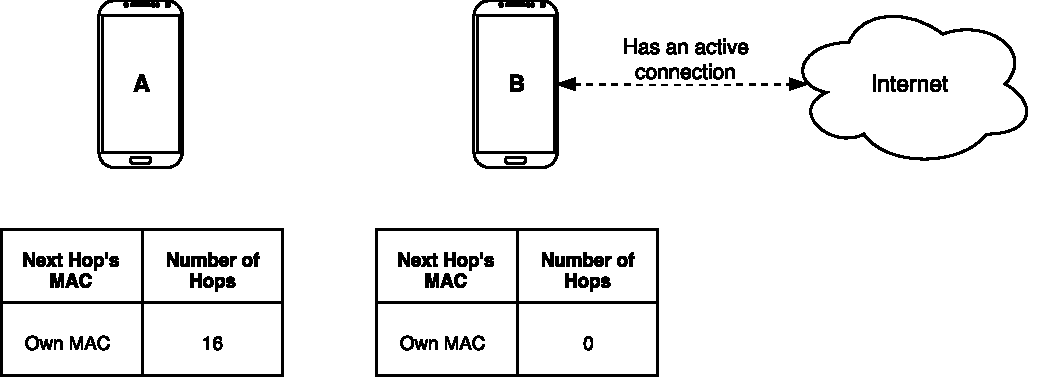
\includegraphics[width=0.9\textwidth]{images/adv_example_1.pdf}}
	\caption{\label{fig:adveg1} Example 1: State of the two devices after the initial step is over}
\end{figure}

A receiver responsible for the management of the Bluetooth discovery process and found peers needs to be created. The management of the discovery process is relatively simple, the receiver needs to be able to assess the discovery process status, \textit{i.e.}, if it is starting, running or finished. The management of peer finding is more complex, the receiver needs to retrieve each peer's information and store it in the peer list previously mentioned. However, before the peer can be instantiated and added as a list item, it is needed to verify if this peer was not previously discovered, avoiding duplicates. Once the discovery is finished the receiver needs to be able to notify the rest of the application that it can proceed with the advertising process.

\begin{figure}[ht]
   \noindent\makebox[\textwidth]
    {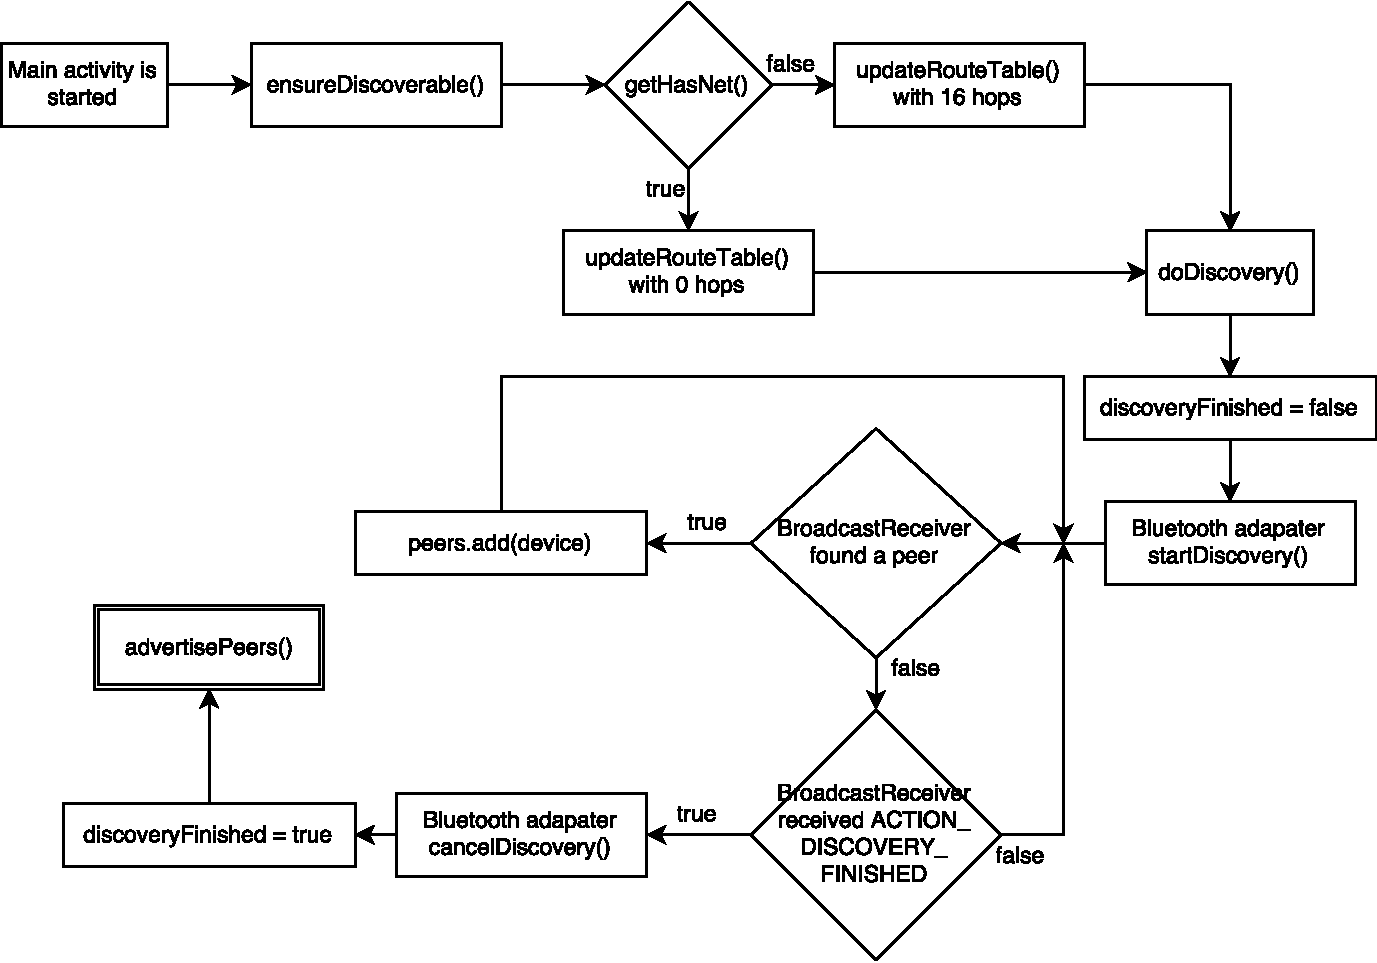
\includegraphics[width=1\textwidth]{images/discovery_flux.pdf}}
	\caption{\label{fig:discflux} Fluxogram of the discovery process}
\end{figure}

In Figure \ref{fig:discflux} it is possible to see sequence of actions the application executes to successfully perform the discovery process.

\subsubsection{Sending an Advertising Message}
\label{subsubsec:sendadv}

The discovered peers are now stored and the device can start the advertising process. The peer list is iterated through and each item is analysed to understand if it should receive an advertisement message or not. The analysis consists of a series of checks to fit the peer into the desired category, in this case a smart phone using the application.

Since the number of Bluetooth devices is growing, it is a plausible possibility that the discovery process found a peer that does not fit into the desired category, such as a sensor or an headset. To avoid this a check is performed to assess if the peer is a smart phone. Overlooking this check can be time and resource costly as the number of attempted connections will increase.

Once the necessary checks are performed and the peer device is eligible to receive an advertisement message, the device attempts to establish a Bluetooth connection, using the mechanism described in \ref{subsec:btconn}. Before sending the advertisement message the application needs to ensure the connection has been successfully established and both devices are ready to write and receive bytes, through the respective streams.

If the conditions to send the message are met the device queries its routing table for the minimum estimated number of hops, explained in Subsection \ref{subsec:disandadv}. To the returned value a unit is added, symbolizing the hop this message will take from sender to receiver. The advertisement is then sent, following the format seen in Figure \ref{fig:advmsg}, where the Bluetooth \gls{MAC} identifier is the device's own \gls{MAC} address.

Before the next iteration through the peer list, a new cycle must be performed to ensure this device does not advertise to a new peer whilst sending a message to the previous one. Thus, the device waits on confirmation that the advertisement message was successfully received by its destination before starting the process again with the next peer.

\begin{figure}[ht]
   \noindent\makebox[\textwidth]
    {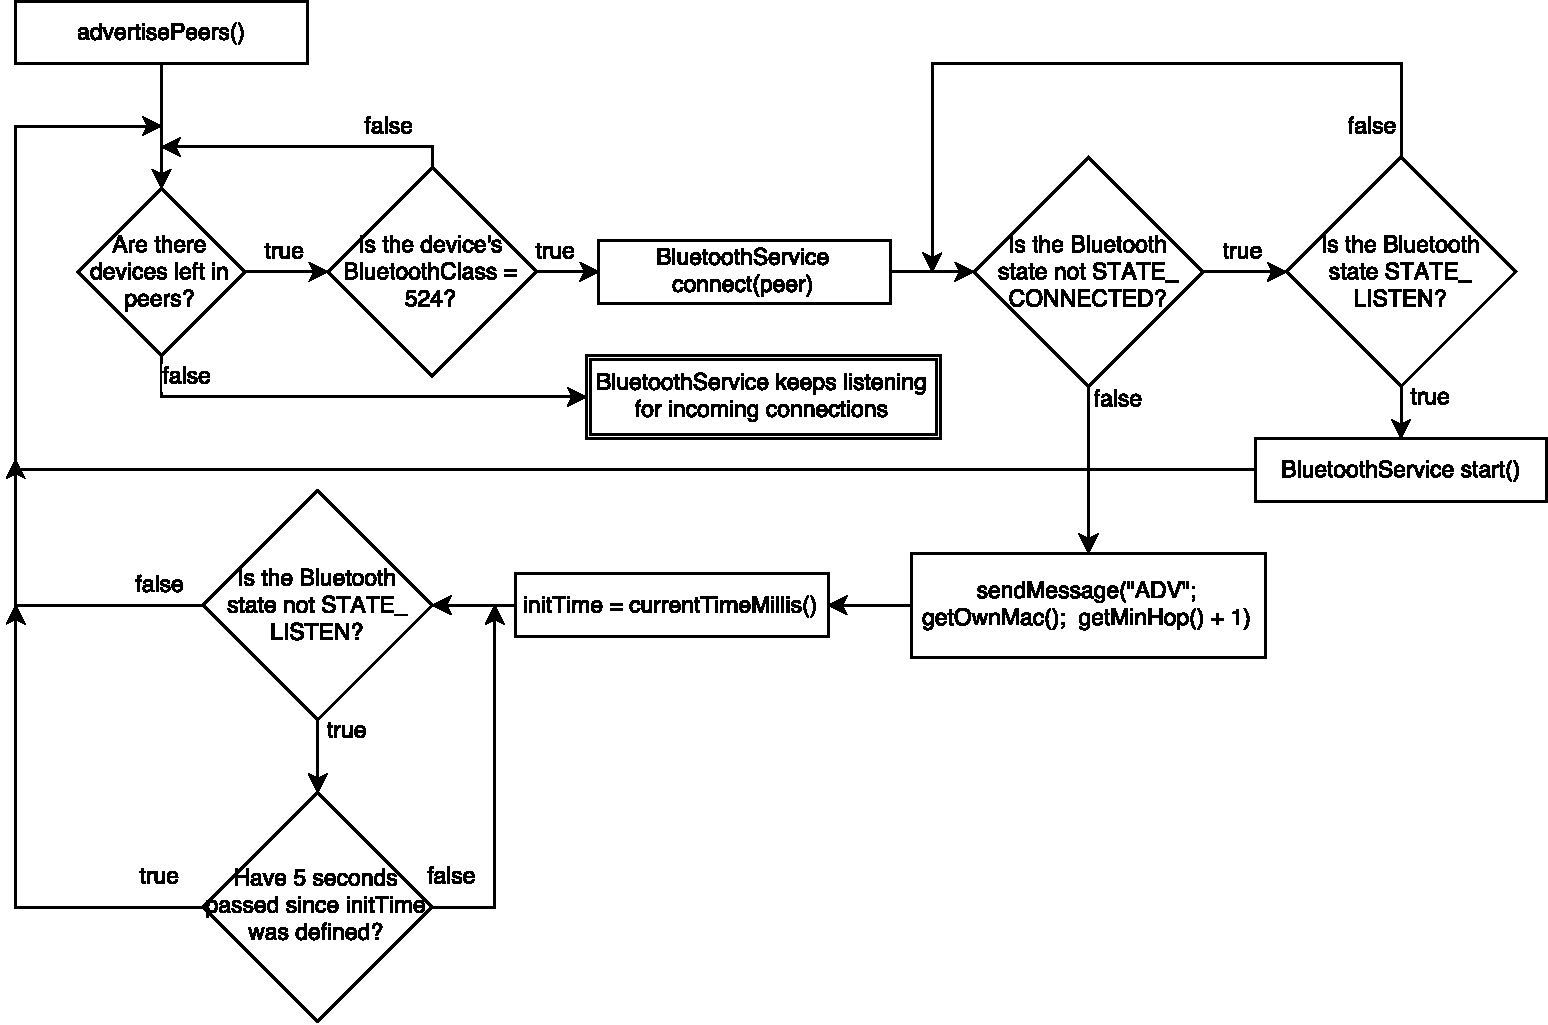
\includegraphics[width=1\textwidth]{images/advertise_flux.pdf}}
	\caption{\label{fig:advflux} Fluxogram of the advertising process from the point of a sender}
\end{figure}

In Figure \ref{fig:advflux} the fluxogram of the advertising process is presented. It shows how the mechanism is executed in a visual manner. Once the process is finished the device remains active waiting for incoming connection requests.

\subsubsection{Receiving an Advertising Message}
\label{subsubsec:rcvadv}

It is now covered how the transmitter of an advertisement message operates. However, to fully understand the advertising process it is necessary to analyse the receiver device and how it handles this message. 

On the receiver device, the \textit{BluetoothService} reads a certain amount of bytes from the input stream, see Figure \ref{fig:inoutstreams}, that need to be transmitted to the main activity. As mentioned before, a handler is used to pass the received bytes from the \textit{BluetoothService} to the main activity. When the main activity is notified of the reception of bytes from a Bluetooth connection it analyses the context of the application, \textit{i.e.}, what format of data is the application expecting to receive at that specific point in time. Since this subsection scope is the advertising process, only text messages are expected to be sent and received.

The connection to the advertiser is no longer required, thus the \textit{BluetoothService} is restarted so the device can start listening to incoming connections. Simultaneously, the received bytes are converted into a text message that will be submitted to analysis, in order to identify what kind of message has the device received, from the different possibilities: advertisement, request, response or fail message.

By comparing the type present in the message, see Figure \ref{fig:advmsg}, the message is identified as an advertisement and submitted to the chain of actions specific to that message type. The first step is to extract the information contained in the message, \textit{i.e.}, the sender's \gls{MAC} address and the estimated number of hops to reach the Internet should a request be sent through that path.

Having these values, the device compares the received estimate with the best from the ones stored in the routing table, process described in Subsection \ref{subsec:disandadv}. If the comparison concludes the received estimate does not top the current best, the routing table is updated with the received estimate and \gls{MAC} address. Otherwise, it means the device has found a better path to reach the Internet, so, once the routing table is updated, the device takes the necessary steps to start a new advertisement process, this time advertising the new best estimate, previously described. 

\begin{figure}[ht]
   \noindent\makebox[\textwidth]
    {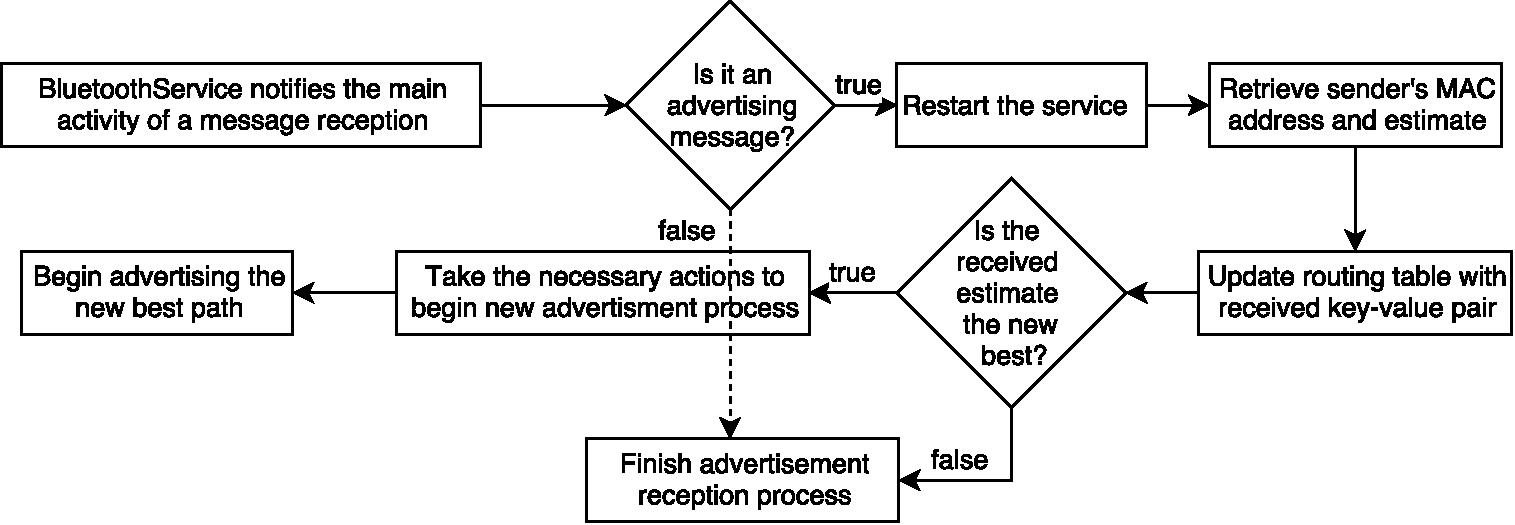
\includegraphics[width=1\textwidth]{images/recv_advertise_flux.pdf}}
	\caption{\label{fig:recvadvflux} Fluxogram of the advertising process from the point of a receiver}
\end{figure}

In Figure \ref{fig:recvadvflux} a fluxogram of the actions taken by the receiver of an advertisement is shown. It reflects what was explained previously in a simplified manner, since some aspects of the mechanism are hidden as they will be discussed later.

\begin{figure}[ht]
   \noindent\makebox[\textwidth]
    {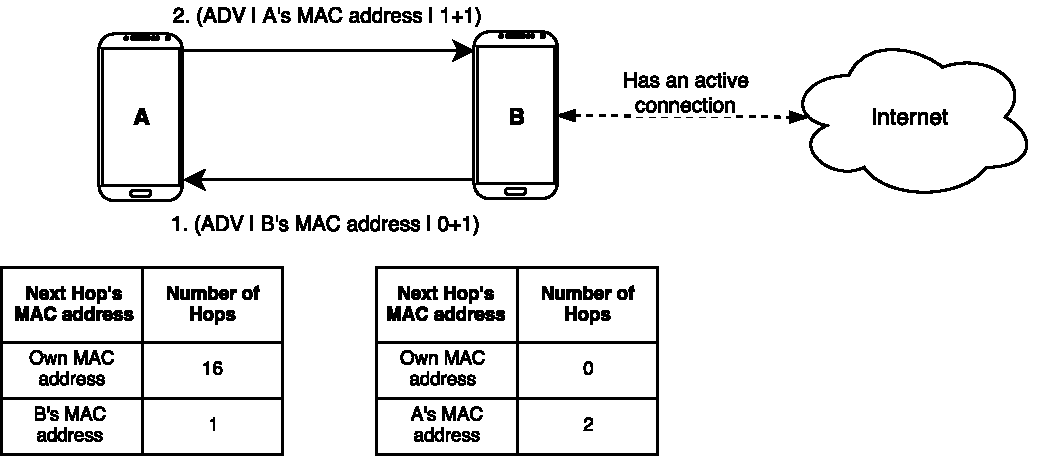
\includegraphics[width=1\textwidth]{images/adv_example_2.pdf}}
	\caption{\label{fig:adveg2} Example 1: State of the two devices after the advertising process is done} 
\end{figure}

To summarize, in Figure \ref{fig:adveg2} the example with devices A and B from Figure \ref{fig:adveg1} is complemented. Now device B has advertised to its peers, which include device A. Upon receiving this message, device A proceeded to store the information in its routing table, followed by and advertise from itself, since the new estimate tops the previous one. After this is concluded both devices have the shown routing tables, and A knows it routes to B, while B routes to itself, since A provides a poorer estimate.

If A advertises first the result would be the same, since when B is advertising A would still receive a better estimate and would advertise again. When B receives the second advertise from A it will overwrite the previous entry, maintaining the same values.

Now it should be clear how the discovery and advertising process is performed and what is the code executed at each time of the process. This is the basis of the next subsection, since without it the devices would not be able to reach the Internet unless they already had the connection.

By giving each device a full view of its vicinity it is possible to establish a network in which every device knows the best path instantly. This is done by what was described above, from discovery to advertisement. The next subsection will refer to the next step, where the devices already have their routing tables populated and are ready to exchange web pages. 

\subsection{Exchange of Web Pages}
\label{subsec:exch}

In this subsection the logic created and implemented to exchange the web pages will be explained in detail, also an example, similar to the previous one, Figures \ref{fig:adveg1} and \ref{fig:adveg2}, will be shown to better demonstrate the processes. Before describing the web page exchange process, it is necessary to explain the routing table related to the exchange of web pages, previously mentioned in Subsection \ref{subsec:disandadv} and referred to as response table.

The main purpose of the response table is to provide a destination for a response message. Once a device has received a request and it has an Internet connection, it should know where to send back the response. This would be easy if only this case applied, it would simply send back the response from where it received the request. But, in the case this device is a "bridge" node, \textit{i.e.}, a node that forwarded a request, it may have received requests from different devices and it still needs to be able to differentiate each message and decide which device to send back the response to.

The response table has a similar structure to the routing table but it serves a different purpose. In Table \ref{tab:rspTables} it is possible to see the structure of the response table.

\begin{table}[ht]
\centering
\bgroup
\def\arraystretch{2.5}
\begin{tabular}{|c|c|}
\hline
\textbf{Message ID} & \textbf{Next hop's MAC} \\ \hline
Message ID \#1 & Device X's MAC \\ \hline
Message ID \#2 & Device Y's MAC \\ \hline
Message ID \#3 & Device Z's MAC \\ \hline
... & ... \\ \hline
Message ID \#9 & Device X's MAC \\ \hline
\end{tabular}
\egroup
\caption{Response table example and format}
\label{tab:rspTables}
\end{table}

Despite having similar structures the two tables store different information: routing table maps a \gls{MAC} address to an estimate whereas the response table maps a message identifier to a \gls{MAC} address. Hence, the necessity of having two distinct tables.

Two main actions must be allowed to be performed in a response table: it must be possible to add new rows, each referring to a specific request and it must be possible to retrieve the next hop's \gls{MAC} address for a certain message identifier. Since the message identifiers are unique, there is no need to update response table rows as there will be no duplicates.

The second action employs a simple logic, given a message identifier the \gls{MAC} address should be returned. Since to a message identifier corresponds a single \gls{MAC} address there should be no problems in the response path. However, in case the requested message identifier is not found in the response table, the application is notified that the response can not be routed due to the lack of a next hop \gls{MAC} address.


\begin{figure}[ht]
   \noindent\makebox[\textwidth]
    {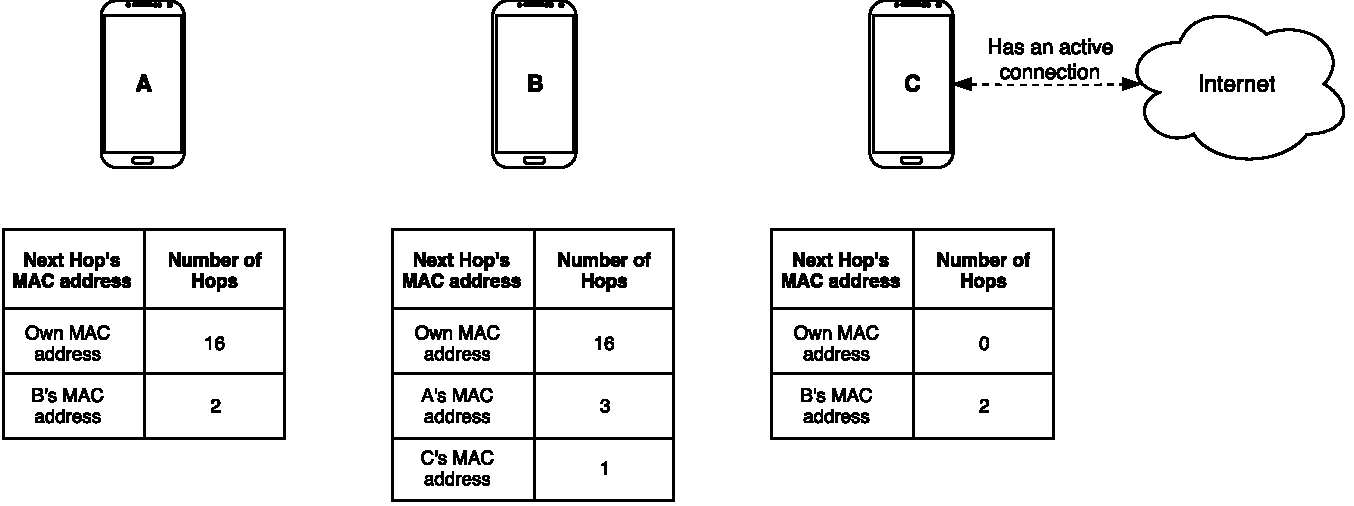
\includegraphics[width=1\textwidth]{images/example_1_0.pdf}}
	\caption{\label{fig:example1.0} Example 2: State of the routing tables of the three devices}
\end{figure}

For the example three devices are used: A, B and C. Where device C has an active Internet connection, as seen in Figure \ref{fig:example1.0}. In the figure it is possible to observe the routing tables of each device after this process is completed. Device A will choose B to send a request and B will choose C, since they provide the best estimates, respectively.


\subsubsection{Sending a Request Message}
\label{subsubsec:sendrqt}

Now that the logic and implementation behind the response table is understood it is possible to explain the mechanism behind the exchange of web pages. This process counts with a number of features that need to be mentioned before further explanation:

\begin{itemize}
	\item  A text area must be defined to enable the input of a \gls{URL} from the application user. This text must be retrievable to form the web page request with the specified \gls{URL}.
	
	\item A button needs to be implemented so the user may notify the application that he/she has finished inputting the desired \gls{URL}. This button will act as a trigger for the application to begin the request sending.
	
	\item A mechanism to manage the actions related to web pages must be created. In this thesis the method found that best fit the requirements was the creation of a \textit{WebView} instance.
	
	\item A handler providing the link between the \textit{BluetoothService} and the main activity, previously mentioned in the context of the advertisement process, that can communicate the bytes received by the service to the rest of the application.
	
	\item Finally, a mechanism to identify how the received bytes should be processed, \textit{i.e.}, what format should they be converted into. This mechanism must also provide a method to identify the received messages between the possibilities and command the application to act accordingly, \textit{i.e.}, follow a specific set of actions for that message type.
\end{itemize}

\begin{figure}[ht]
   \noindent\makebox[\textwidth]
    {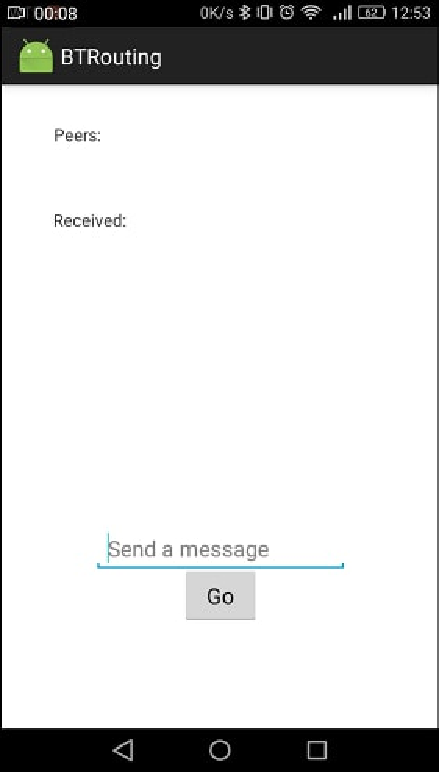
\includegraphics[width=0.3\textwidth]{images/initScreen.pdf}}
	\caption{\label{fig:initScreen} User interface for the sending of request messages}
\end{figure}

In Figure \ref{fig:initScreen} it can be seen the user interface of the main activity, it has five main elements: a place where the \textit{peers} list is displayed, at the top. The received messages, this is an optional element and used for debugging as it would incur in severe security issues. A text area, as mentioned before, allowing the user to input the web page he/she desires and to capture this input to be processed. And a button to notify the activity that the process of requesting that specific web page must be initiated.

Assuming the device already established the best route to reach the Internet, \textit{i.e.}, its routing table is populated, the journey of the web page request from the user input to the display of the response will be explained. Starting from the user input, has mentioned above a button and a text area are created, forming a user interface allowing the sending of requests based on the user input.

\begin{figure}[ht]
	\noindent\makebox[\textwidth]
	{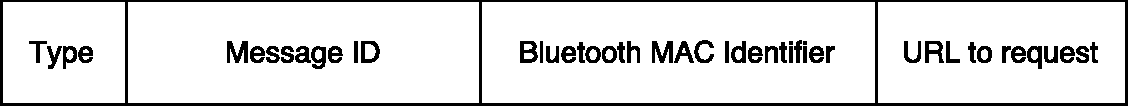
\includegraphics[width=0.9\textwidth]{images/rqtmessage.pdf}}
	\caption{\label{fig:rqtmsg} Request message format}
\end{figure}

In Figure \ref{fig:rqtmsg} a generic request message is shown. Its format does not differ much from the one presented in Figure \ref{fig:advmsg}. However two new fields are introduced: the \textit{Message ID}, a unique identifier representing each message that will be useful to keep track of what is each message's payload and sender and the \textit{\gls{URL} to request} is the web page's \gls{URL} the user is trying to access, it is considered to be the payload of the message.

The web page request process may be initiated by two different events: when the user inputs an \gls{URL} and presses the "Go!" button or when the device receives a request and its next action is to forward it to the next hop.

Beginning by the first event, the button needs to act as a trigger for the application. To achieve this the logic to begin the request process when the button is pressed must be implemented. This trigger must also be able to provide the input text by the user, containing the web page to be requested. Having the \gls{URL} the request process can be initiated. Note that this process must differentiate the two possible events that lead to it, since they incur into different workflows.

Assuming the originating event is correctly identified and the process is aware that it was initiated by user interaction, the first action is to retrieve the next hop's \gls{MAC} address, to whom the device shall send its request. This can be achieved by using the routing table features, see Subsection \ref{subsec:disandadv}, that provide the best path's next hop.

If the routing table query does not return a valid \gls{MAC} address the user must be notified of the request failure. However, if a valid \gls{MAC} address for the next hop is returned, the device attempts to establish a connection with the next hop, following the same mechanism as in the advertising process. Should the connection attempt fail the user is also notified of the request failure, allowing him/her to restart the request process, and the \textit{BluetoothService} restarted to keep the device listening to incoming connections.

If the connection is successfully performed, the application may proceed to the generation of the request message to be sent. The message is composed by four sections previously defined, see Figure \ref{fig:rqtmsg}. 

\begin{itemize}
	\item The \textit{Type} corresponds to the message type and is already known, as the button clicking triggered the request sending process, being populated accordingly.
	
	\item To fill the \textit{Message ID} section a message identifier must generated to distinguish this request between the others that may be sent throughout the network. To do this, a random number is generated between -2\textsuperscript{31} and 2\textsuperscript{31}, providing a wide range of possibilities and minimizing immensely the occurrence of duplicates.
	
	\item The \textit{Bluetooth \gls{MAC} Identifier} address is the device's own \gls{MAC} address and it will allow the receiver to correctly assess the response's path.
	
	\item Finally, the \textit{\gls{URL} to request} is populated with the text retrieved from the user input, seen in Figure \ref{fig:initScreen}.
\end{itemize}

Once the request message is sent the application updates its response table with the generated message identifier and the \gls{MAC} address of the sending device, \textit{i.e.}, its own, as a key-value pair. With this mechanism the device is able to assess if it is the destination of a certain response or if it is a "bridge" node and needs to forward the response to the next hop. This assessment will be presented and explained in \ref{subsubsec:rcvrqt}.

If the device is not deemed as the owner, there is no random identifier generation, since the value will be retrieved from the received request message. Also, the response table is not updated because this will be done during the receiving process, the next focus. Despite that, the connection is attempted, same as before.

However, if the connection establishment fails the user is not notified, since this request was not originated by him/her. In this case, the device queries the response table for the \gls{MAC} address mapped by the request message identifier, corresponding to the device that sent/forwarded the request to this node. A failure notice is then sent to that device, with the intent of notifying the request originator of the inability to forward the request until it reaches the Internet.

If the connection is successfully established, the message is sent as before with the slight difference that the message identifier and the \gls{URL} to be requested are retrieved from the values encapsulated in the received request message, see Figure \ref{fig:rqtmsg}.

\begin{figure}[ht]
   \noindent\makebox[\textwidth]
    {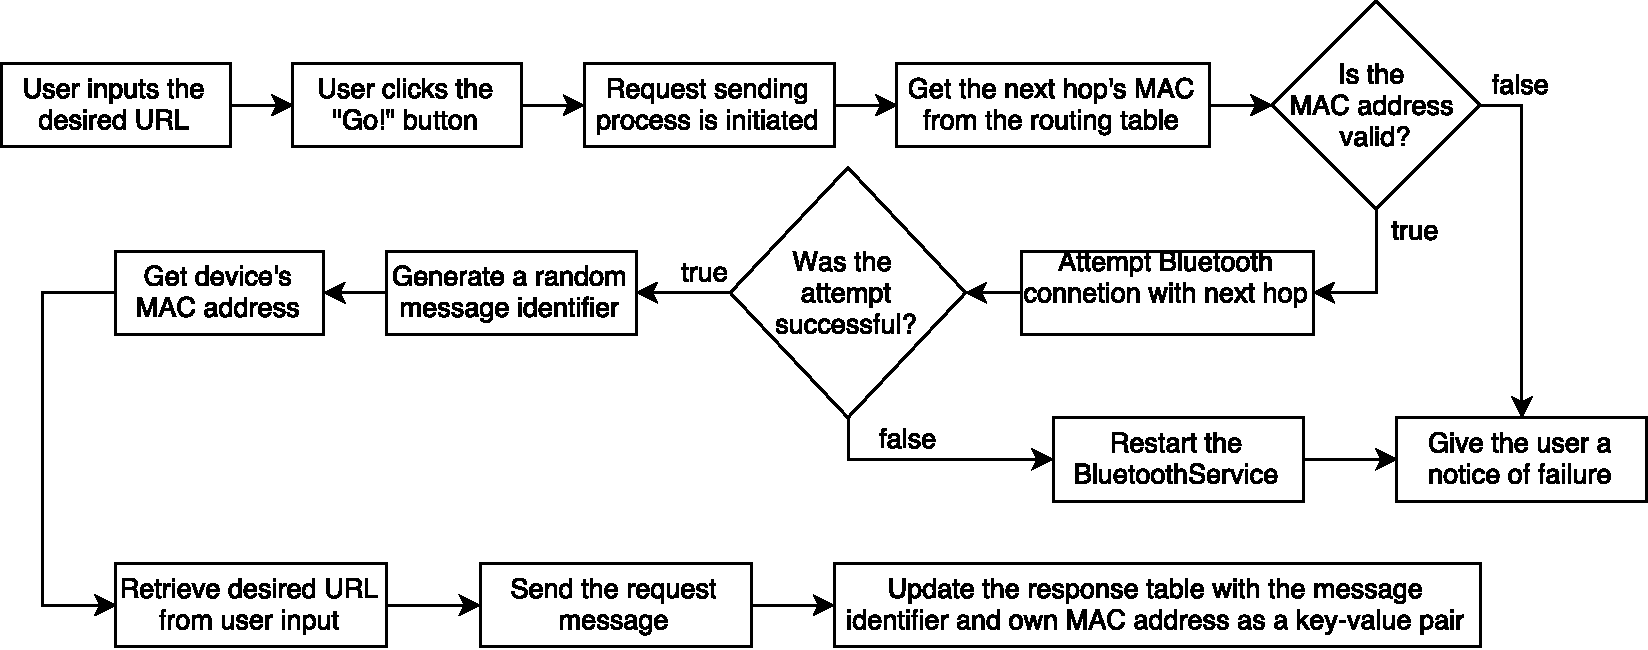
\includegraphics[width=1\textwidth]{images/rqtflux.pdf}}
	\caption{\label{fig:rqtflux} Fluxogram of the request sending process triggered by user input}
\end{figure}

In Figure \ref{fig:rqtflux} a fluxogram representing the process described above is presented. It provides a visual overview of the application workflow when user input triggers the request sending mechanism. Once the process is finished the device keeps listening to incoming connections.

\subsubsection{Receiving a Request Message}
\label{subsubsec:rcvrqt}

The request receiving process is similar to the advertise, the receiver connects to the sender and receives the bytes from the request sent. As before, the bytes are transmitted from the \textit{BluetoothService} to the main activity, through a \textit{MESSAGE\_READ Message} and the \textit{mHandler} receives them. After comparing the received \textit{Message} to the possible types, explained in Subsection \ref{subsubsec:rcvadv}, and concluding it is a \textit{MESSAGE\_READ} the \textit{Handler} converts them to a \textit{String}. Since the newly created \textit{String} is not a response, the \textit{BluetoothService} is restarted and \textit{analyzeMessage()} is called taking as argument the \textit{String}.

In \textit{analyzeMessage()} the argument \textit{String} is compared to the possible message types, \textit{ADV}, \textit{RQT}, \textit{RSP} and \textit{FAIL}. It will now be identified as a response, due to the analysis of the message type, see Figure \ref{fig:rqtmsg}, and immediately the message identifier is saved in the variable \textit{msgID}.

In the request sending process it was mentioned that, in case the device was not the owner of request, it would not update the response table. This was due to the fact that, for the devices that are not the owners of the request, this process is done here, in \textit{analyzeMessage()}. So, the routing table is updated with the message identifier and \gls{MAC} address of the sender, retrieved from the message.

Two different approaches can now be taken: one regards the devices with Internet connection and the other the devices without one. To define which approach is taken by the device a quick check of the Internet connection status is performed, via the method \textit{getHasNet()}. If the result is false, meaning the device has no Internet connection, the request will be forwarded to the next hop to reach a device with Internet. To do this, the device calls \textit{sendRequest()} with arguments: false, the message identifier, retrieved from the received message and the \gls{URL} requested, also retrieved from the message. The method follows the same steps as before, described in \ref{subsubsec:sendrqt}.

If the result of the \textit{getHasNet()} query returns true, it means the device has an Internet connection and, as such, it is a final destination. This means the device will now be the communication link with the Internet and it needs to retrieve the requested web page and send it backwards until it reaches the owner of the request. This process begins by calling the method \textit{getPage()}, that receives the requested \gls{URL} and the message identifier, both retrieved from the received message.

In \textit{getPage()} the web page is downloaded via the \textit{WebView}, mentioned in \ref{subsubsec:sendrqt}. A new \textit{WebViewClient} is created, see \cite{webview} for documentation on \textit{WebView} and its features, such as the \textit{WebViewClient}. This client is different from the usual, since the device does not want to display the downloaded page.

The methodology to save the web page had several possibilities, such as saving the web page as an image, saving only the \textit{HTML} content or saving each element of the page individually. The first two methods are not complete, meaning the web page could lose some of its features, \textit{e.g.} dynamic images, search fields, \textit{etc.}. The third method would fully download the web page, however it would require additional logic to save the different elements in the same directory and to arrange them to re-create the web page with its initial format.

The method \textit{saveWebArchive()} provides a complete solution to this problem, it is a method specific to the \textit{WebViewClient}'s class, see \cite{webview} and it solves the problem of third method, since it downloads each element but compiles them in a web archive, that can be decompressed easily by \textit{WebView}. Thus, it proved to be the better solution for this problem.

To implement this methodology, the method \textit{onPageFinished()}, from \textit{WebViewClient}'s class, is overwritten. This method is used to do something after the web page is finished loading. So, a new \textit{File} is created in the application's directory, with the name "file.mht". If the file creation succeeds, the web page is downloaded and saved in the created file, via \textit{saveWebArchive()}. In order to guarantee the web page is downloaded and saved before the response is set, a \textit{waitForWebPage} downloader is created and executed.

The \textit{waitForWebPage} class can be seen in appendix \ref{appendix:BtActivity} and was created with the sole purpose of guaranteeing the web page transfer is completed before the response is sent. If this check is not performed, it is possible that, for large web pages, the response file will be incomplete and thus not displaying correctly the requested \gls{URL}.

It extends an \textit{AsyncTask}, used to perform background operations and send the results to the main thread, see \cite{async} for the full documentation. It starts by creating a variable \textit{file} that will contain the address where the web page will be saved. The method \textit{doInBackground()} is overwritten, as it always has to be in an \textit{AsyncTask}, since it contains what operations to be performed.

In this method it is continuously checked if the variable \textit{file} has a size bigger than 0 bytes. Whenever this condition is verified, it means the web page was saved successfully. The \textit{onPostExecute()} method, used to send the results to the main thread, is also overwritten and, once this thread reaches this point, it means the device is ready to send the response, so \textit{sendResponse()} is called.

\begin{figure}[ht]
   \noindent\makebox[\textwidth]
    {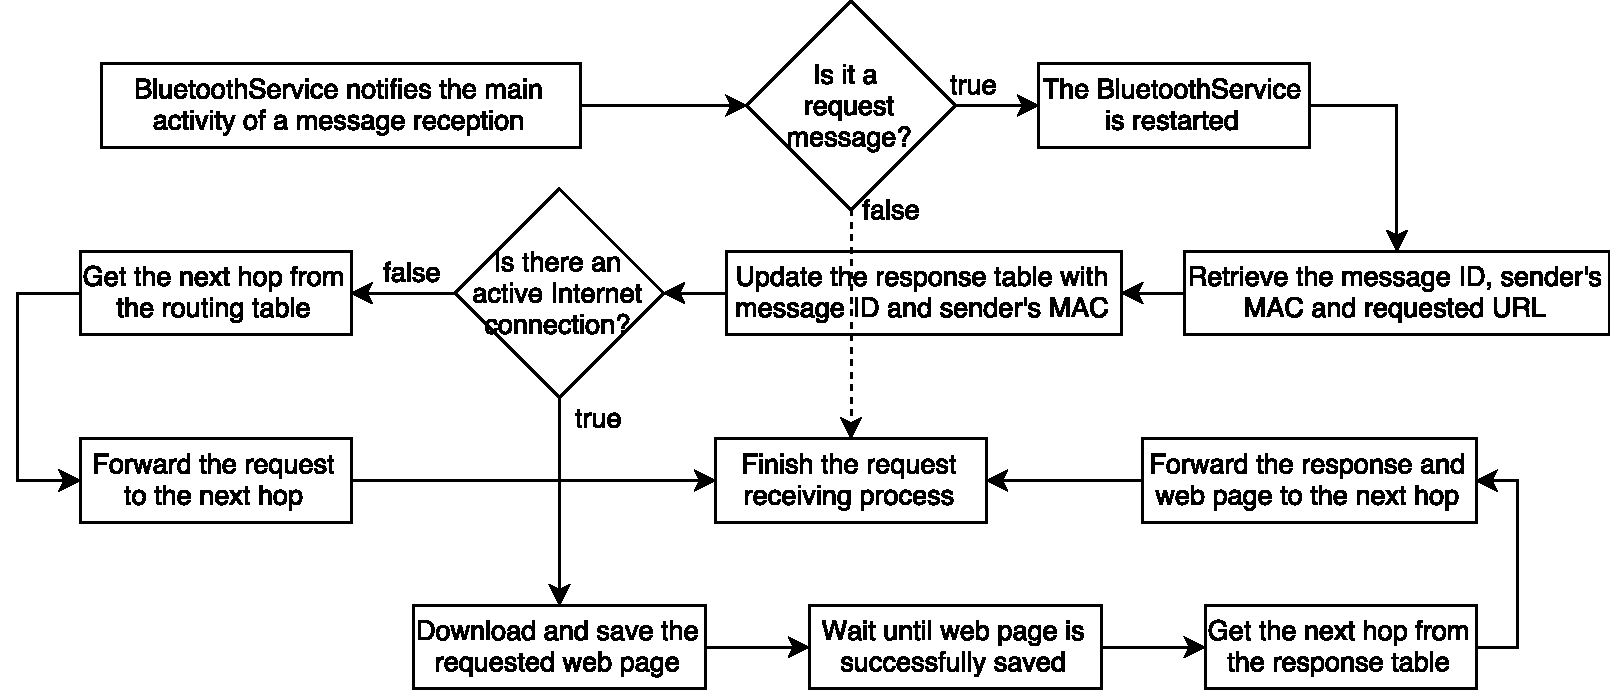
\includegraphics[width=1\textwidth]{images/rqt_rcv_flux.pdf}}
	\caption{\label{fig:rqtrcvflux} Fluxogram of the request receiving process}
\end{figure}

In Figure \ref{fig:rqtrcvflux} it is possible to see a fluxogram of this process. The process, as shown in the figure, ends either with sending a new response or a new request, depending on whether the device has Internet connection or not, respectively.

\begin{figure}[ht]
   \noindent\makebox[\textwidth]
    {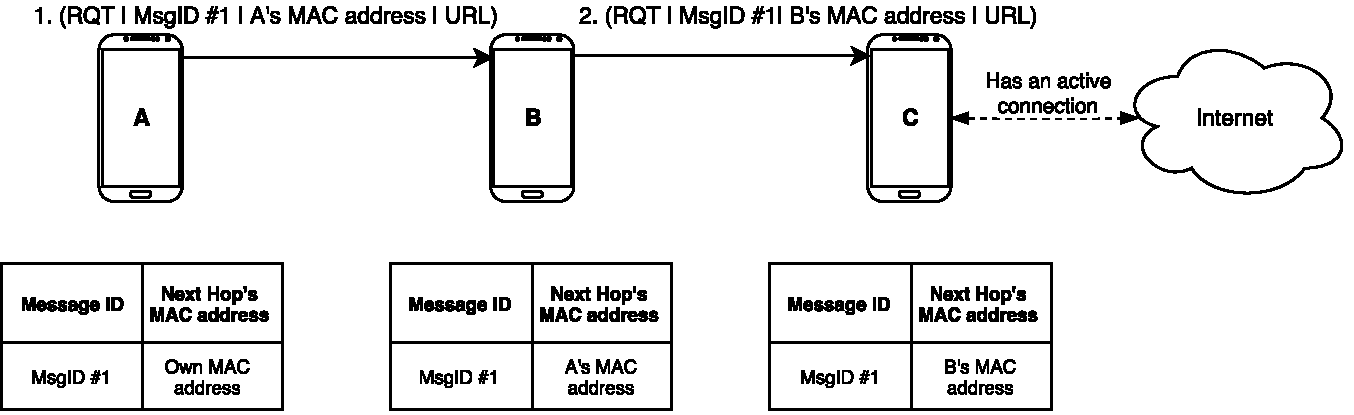
\includegraphics[width=1\textwidth]{images/example_1_1.pdf}}
	\caption{\label{fig:example1.1} Example 2: Request sending and receiving process}
\end{figure}

Resuming the example in Figure \ref{fig:example1.0} and supposing the user from device A wants to request a \gls{URL} and inputs it correctly, the device will follow the steps explained in Subsection \ref{subsubsec:sendrqt} and check the routing table to establish the next hop. Also its response table will be filled during this action, since it is the owner of the request.

Once that process is completed and the message reaches device B it will update its routing table with the newly received request. After that it checks its own routing table and assesses if it should forward the request or download the page. Since the device does not have an active connection the first option will chosen and the request forwarded to C.

Finally, upon receiving the request, device C will update its own response table with the received message identifier and B's \gls{MAC} address. Having an Internet connection the device will download the web page.

In Figure \ref{fig:example1.1} it is shown the above described, as well as the three response tables from the devices once the requests are all sent and the web page downloaded.

\subsubsection{Sending a Response Message and Web Page}
\label{subsubsec:sendrsp}

Once the web page is successfully saved in the device it is possible to send the response back until the owner of the request receives the requested web page. As seen before, \textit{sendResponse()} is called in \textit{onPostExecute()} and it is used to send a response to the next device.

It receives as parameter the message identifier, so that the \gls{MAC} address of the next device can be retrieved from the response table. Thus, having the message identifier and through the method \textit{getRspHop()}, the device retrieves the next hop's \gls{MAC} address. Should the result of this call be null, the response will not be sent. If the result returns a valid \gls{MAC} address, the connection process is performed, along with the cycle to ensure the connection is successful, described in Subsection \ref{subsubsec:sendadv}.

\begin{figure}[ht]
   \noindent\makebox[\textwidth]
    {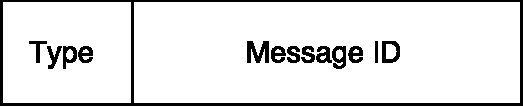
\includegraphics[width=0.4\textwidth]{images/rspmessage.pdf}}
	\caption{\label{fig:rspmsg} Format of a response message}
\end{figure}

Finally, if all the above goes as planned and succeeds, the response is sent with the format seen in Figure \ref{fig:rspmsg}, with "RSP" as \textit{Type} and the received argument \textit{msgID} as \textit{Message ID}.

The next step is to send the actual web page to the next hop, but first the sender needs to ensure the response was correctly sent. This is done by the \textit{Handler}, explained in Subsection \ref{subsubsec:sendadv}. The \textit{Message} type \textit{MESSAGE\_WRITE} is used for this, since it returns the bytes sent from the device and convert them to a \textit{String}. If the converted \textit{String} is a response message the application concludes the process is completed correctly and proceeds to call the method \textit{sendFile()}.

The \textit{sendFile()} method is called when the device is ready to sent the web page bytes to the next hop. It begins by creating a variable \textit{file}, pointing to the file in the application storage that contains the web page. The size of that file is retrieved through \textit{file.length()} and an array of bytes is created with that same size. This array of bytes will be the place where the web page will be transferred, from the internal storage to the application.

In order to transfer the web page from the file, in the internal storage, to the application a \textit{BufferedInputStream} is used, see \cite{bis} for more documentation on this class. This \textit{BufferedInputStream} instance takes the bytes from the variable \textit{file}, previously described and saves them in the array of bytes, it is then closed to avoid memory leaks.

Once the bytes are transferred to the application the device needs to send them to the next hop, since the connection is still opened, for reasons that will be explained in the next subsection, it is possible to send the bytes without the logic to connect to the next hop. The method \textit{writeFile()} from \textit{BluetoothService} is called and the file bytes is transferred to the next hop as described in Subsection \ref{subsubsec:connected}.

The method gets the number of bytes to be sent and divides that size by 990 bytes, getting the number of chunks that need to be sent to the next hop. It then proceeds to send each chunk with a length of 990 bytes, until it reaches the last chunk, sending the remaining bytes.

\begin{figure}[ht]
   \noindent\makebox[\textwidth]
    {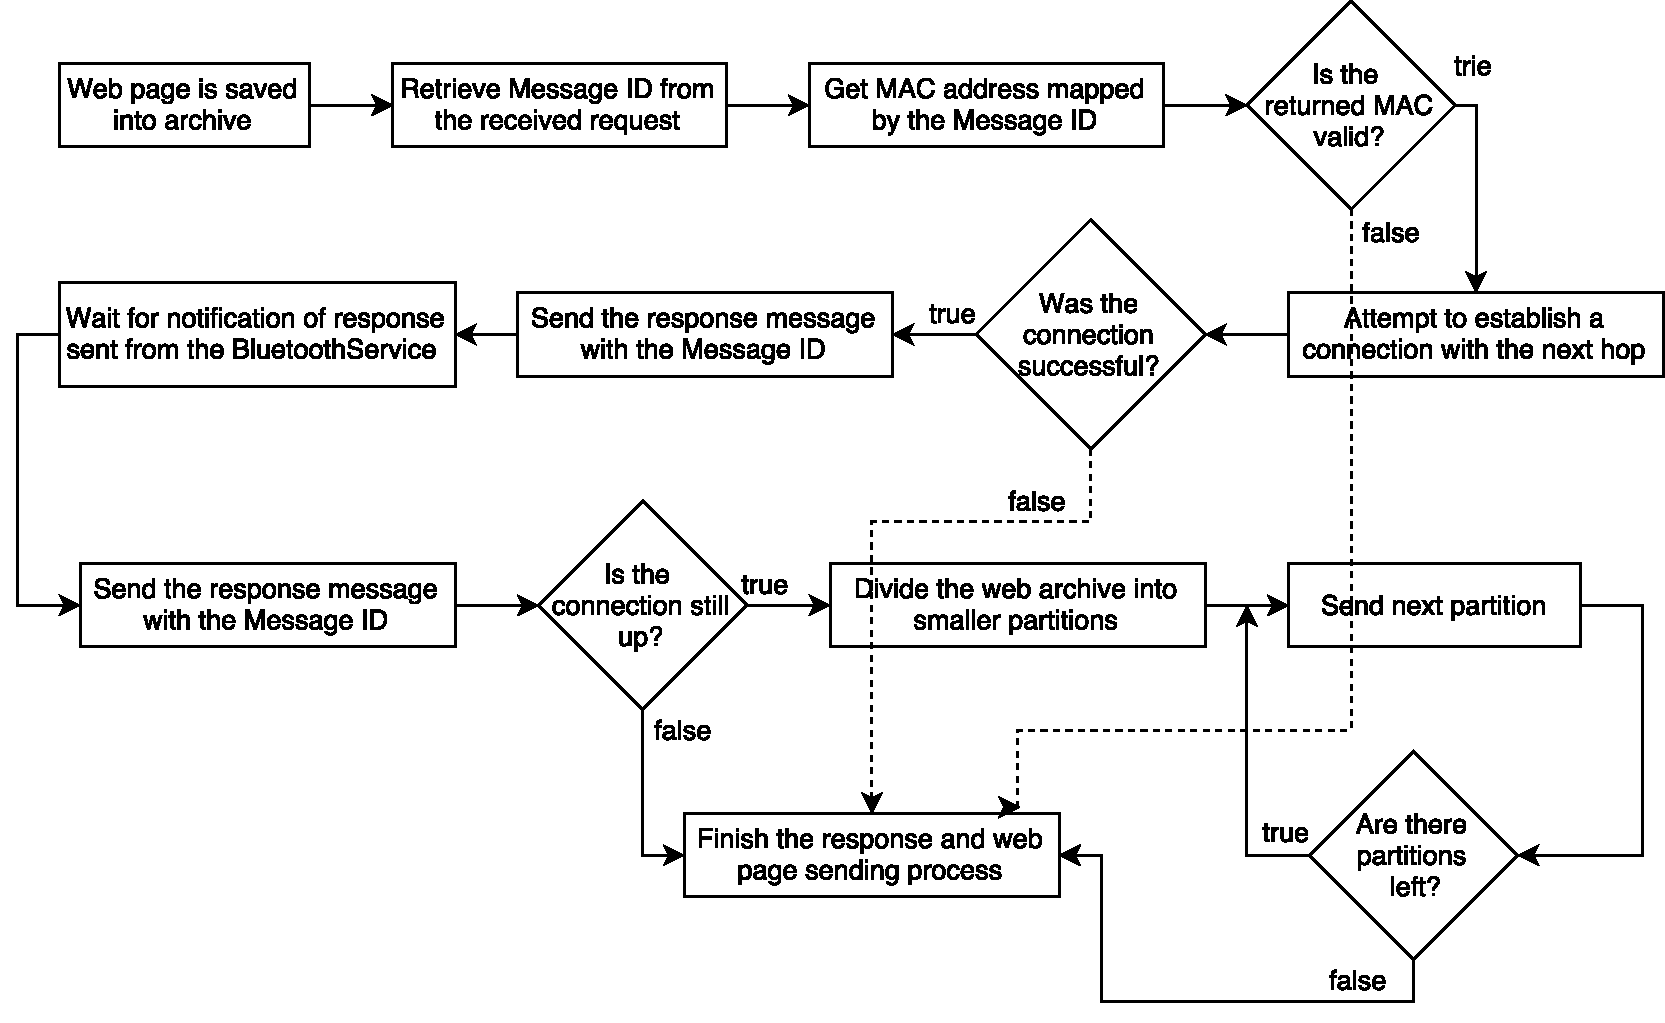
\includegraphics[width=1\textwidth]{images/send_rsp_flux.pdf}}
	\caption{\label{fig:rspsendflux} Fluxogram of the response and web page sending process}
\end{figure}

In Figure \ref{fig:rspsendflux} a fluxogram of the response sending response is presented. It shows the process from the saving of the web page to the sending of the same. As previously described the fluxogram ends by dropping the message if there is no valid next hop for that message identifier, by restarting the \textit{BluetoothService} if the connection fails, or by sending the full web page as expected.

\subsubsection{Receiving a Response Message and Web Page}
\label{subsubsec:rcvrsp}

In the receiver side, the web page and response are received and the device must assess if it is the final destination or if it is a relay node for a different device, in which case the web page will not be displayed, but the response and web page are forwarded.

This process begins in the \textit{Handler}, where the notification is notified that a message as been received by a \textit{MESSAGE\_READ}. The received message is compared with the possible types and, since it is a response message, it is identified as such. In the case of a response, the \textit{BluetoothService} is not restarted, since the device benefit from keeping the connection active to avoid further delays in re-connecting to receive the web page, also mentioned in Subsection \ref{subsubsec:sendrsp}. Instead, the \textit{BluetoothService}'s variable \textit{fileReady} is set to "true", meaning the device is has received a response message and is ready to receive the associated web page.

The message is then sent to method \textit{analyzeMessage} as a \textit{String}, where the message identifier will be saved to \textit{msgID}, retrieved from the response message, see Figure \ref{fig:rspmsg}. Having the message identifier the method compares the device's \gls{MAC} address to the one returned from \textit{getRspHop()} for that same message identifier. If both addresses match the device is the destination and the owner of the request, so the web page will be displayed. Otherwise, the response will be forwarded to the next destination.

The sender will then proceed to transfer the web page bytes from one device to another. At this point the receiver is expecting a file, since the variable \textit{fileReady} is set to "true". This shifts the \textit{BluetoothService} reception logic from receiving a \textit{String} to receiving a web page, see Subsection \ref{subsubsec:connected} for more details on this logic.

A variable \textit{output} is created, where each 990 bytes chunk is saved. When the transfer reaches the last chunk, identified by its size, which will be smaller than 990 bytes, the information contained in this variable is passed to a byte array, that will be sent back to main activity via a \textit{FILE\_READ Message}.

Once the main activity's \textit{Handler} receives this notification it copies the bytes received from \textit{BluetoothService} to a file in the application's directory. The \textit{BluetoothService} is restarted and the variable \textit{fileReady} is set to "false", as the device does not expect to receive anymore files for the time being. A new comparison between the device's own \gls{MAC} and the result of \textit{getRspHop} for that specific message identifier is made. If the result is false, meaning the device is not the destination, the response is forwarded through \textit{sendResponse}, with the corresponding message identifier, see \ref{subsubsec:sendrsp} for information on this process.

However, if the device is deemed the owner of the original request and thus the destination of the web page, the method \textit{loadPage()} is called, were the logic to display the web page is performed. First the \textit{WebView} instance is set to load web pages first from cache instead of directly trying to access the network, via \textit{setCacheMode(WebSettings.LOAD\_CACHE\_ELSE\_NETWORK)}, see \cite{webview} for more documentation. It is followed by setting the \textit{WebView}'s visibility to \textit{VISIBLE}.


There is one important aspect of this application that was not yet discussed. When the requester receives the web page, it might be needed to request multiple pages, for instance in a Google search, the user requests the front page and then inserts its query and a subsequent page is requested. This logic has to be reflected in the application for it to be deemed useful and usable. If the user had to go back and input each \gls{URL} by itself the application would have no real application.

\textit{WebViewClient}'s class may have a solution to this problem. The class method \textit{onReceivedError} is triggered whenever the \textit{WebView} receives an error, meaning it is possible that, whenever a "no Internet" error is received logic can be created in order to prevent the \textit{WebView} to display that error and instead create a request with the \gls{URL} that returned the error.

To do that, this method is overwritten, beginning by loading the page "about:blank", a page composed of a white screen, in order to avoid the user seeing the error page. A request message is then sent, via \textit{sendRequest} with the arguments: "true", -1 and the \gls{URL} that originated the error, see \ref{subsubsec:sendrqt} for a reminder on how this process is carried. Alongside this, a new \textit{WebChromeClient} is assigned, to handle the display of the web page, see \cite{webview} for more information on this class.

Finally, the web page is displayed via the \textit{WebView} method \textit{loadURL}, which for Android versions superior to 5.1 works perfectly. However if the device's Android version is prior to that the archive where the web page is saved has a different formatting and, as such, needs to be compiled again, via \textit{loadArchive()} by calling \textit{WebView}'s method \textit{loadDataWithBaseURL()} with data retrieved from the saved archive with the methods \textit{getStringFromFile()} and \textit{convertStreamToString()}, taken from \cite{stack}.

\begin{figure}[ht]
   \noindent\makebox[\textwidth]
    {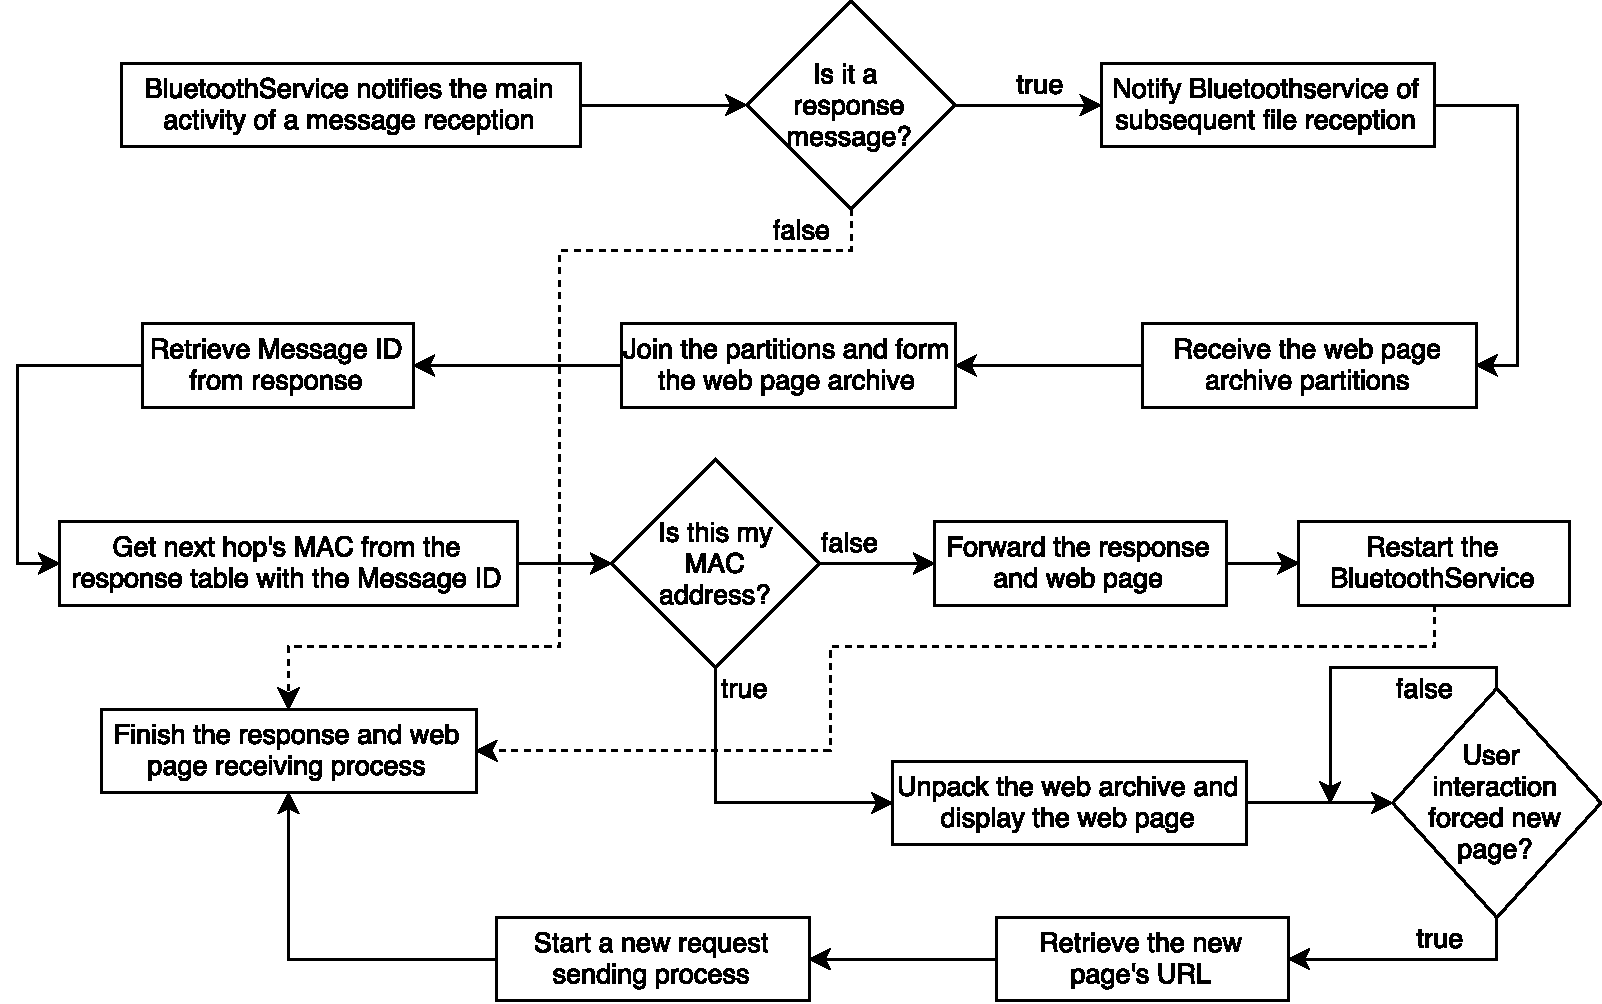
\includegraphics[width=1\textwidth]{images/rcv_rsp_flux.pdf}}
	\caption{\label{fig:rsprcvflux} Fluxogram of the response and web page receiving process}
\end{figure}

In Figure \ref{fig:rsprcvflux} a simplified fluxogram of the response and web page receiving process is shown. It is possible to visualize the file receiving logic, as well as the different possibilities for the receiver of the response: forwarding the response or displaying the web page. It is also shown the logic behind the multi web pages request.

With this implementation the user is capable of seeing the request web pages and navigate through those pages without having to manually send each request.

To finalize the example from Figures \ref{fig:example1.0} and \ref{fig:example1.1}, device C, after finishing the download of the web page, will check its response table and send a response message to device B, which is the next hop retrieved for that specific message identifier \textit{MsgID \#1}. The response is followed by the web page archive, previously downloaded, as described in Subsection \ref{subsubsec:sendrsp}.

Device B receives the response and the web page following the steps previously explained in Subsection \ref{subsubsec:rcvrsp} and checks its response table for that message identifier. Device A's \gls{MAC} is returned from that query and that's the destination for B's response, so device B sends the response and web page to A.

A receives the response and web page following the same steps as B. However, when checking the next hop for that message identifier device A gets its own \gls{MAC} address and concludes it is the final destination for that response, proceeding to display the web page requested by the user, as described this subsection.

\begin{figure}[ht]
   \noindent\makebox[\textwidth]
    {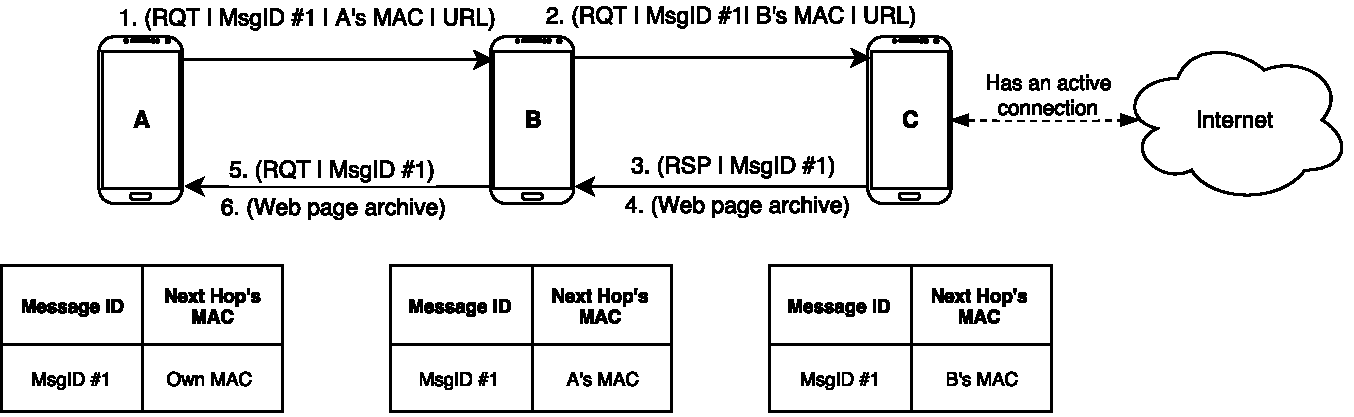
\includegraphics[width=1\textwidth]{images/example_1_2.pdf}}
	\caption{\label{fig:example1.2} Example 2: Sending and receiving of response messages and web pages}
\end{figure}

Figure \ref{fig:example1.2} illustrates this example and messages exchanged between the three devices, as well as the response tables, previously established in Figure \ref{fig:example1.1}.











